
\section{Results}

\subsection{Calculation of the Monthly mean of Chlorophyll-a Concentration in the East Sea (Sea of Japan)}

The monthly-mean chlorophyll-a concentration of LAC from 2003 to 2006 is shown in Figure \ref{fig:monLAC01}. - Figure \ref{fig:monLAC03}. The monthly-mean chlorophyll-a concentration of GAC from 2003 to 2006 is shown in Figure \ref{fig:monGAC01} - Figure \ref{fig:monGAC03}. In these figures, the grey area is land of western part of Korean and southeastern part of Japan. Red area refers to relatively higher concentration compared to the blue area as it is shown at the color bar. Spring (March, April, May) and fall (October, November) show high concentration. The black area is part with no data due to cloud coverage or satellite failures. 

start 박기현
The monthly-mean chlorophyll-a concentration of LAC from 2003 to 2006 is shown in Figure \ref{fig:monLAC01}. - Figure \ref{fig:monLAC03}. The monthly-mean chlorophyll-a concentration of GAC from 2003 to 2006 is shown in Figure \ref{fig:monGAC01} - Figure \ref{fig:monGAC03}. In these figures, the grey area is land of western part of Korean and southeastern part of Japan. Red area refers to relatively higher concentration compared to the blue area as it is shown at the color bar. Spring (March, April, May) and fall (October, November) show high concentration. The black area is part with no data due to cloud coverage or satellite failures. 
end 박기현

\begin{figure}[p]
	\centering
	\includegraphics[width=1.0\textwidth]{monLAC01}\\
	\caption{The monthly-mean chlorophyll-a distribution in the East Sea (Sea of Japan), LAC. From 2003 to 2006, January to April. The unit of the color bar is $\rm mg/m^3$.}
	\label{fig:monLAC01}
\end{figure}


\begin{figure}[p]
	\centering
	\includegraphics[width=1.00\textwidth]{../images/monLAC02}\\
	\caption{The monthly-mean chlorophyll-a distribution in the East Sea (Sea of Japan), LAC. From 2003 to 2006, May to August. The unit of the color bar is $\rm mg/m^3$.}
	\label{fig:monLAC02}
\end{figure}

\begin{figure}[p]
	\centering
	\includegraphics[width=1.00\textwidth]{../images/monLAC03}\\
	\caption{The monthly-mean chlorophyll-a distribution in the East Sea (Sea of Japan), LAC. From 2003 to 2006, September to December. The unit of the color bar is $\rm mg/m^3$.}
	\label{fig:monLAC03}
\end{figure}


\begin{figure}[p]
	\centering
	\includegraphics[width=1.0\textwidth]{../images/monGAC01}\\
	\caption{The monthly-mean chlorophyll-a distribution in the East Sea (Sea of Japan), LAC. From 2003 to 2006, January to April. The unit of the color bar is $\rm mg/m^3$.}
	\label{fig:monGAC01}
\end{figure}


\begin{figure}[p]
	\centering
	\includegraphics[width=1.00\textwidth]{../images/monGAC02}\\
	\caption{The monthly-mean chlorophyll-a distribution in the East Sea (Sea of Japan), LAC. From 2003 to 2006, May to August. The unit of the color bar is $\rm mg/m^3$.}
	\label{fig:monGAC02}
\end{figure}


\begin{figure}[p]
	\centering
	\includegraphics[width=1.00\textwidth]{../images/monGAC03}\\
	\caption{The monthly-mean chlorophyll-a distribution in the East Sea (Sea of Japan), LAC. From 2003 to 2006, September to December. The unit of the color bar is $\rm mg/m^3$.}
	\label{fig:monGAC03}
\end{figure}


\newpage
 
\subsection{The Annual Variability of Chlorophyll-a Concentration in the East Sea (Sea of Japan)}
 

%%%%%%%%%%%%%%%%%%%%%%%%%%%%%%%%%%%%%%%%%%%%%%%%%%%%%%%%%%%%%%%%%%%%%%%%%%   
% \begin{figure}[b]
% 	\centering
% 	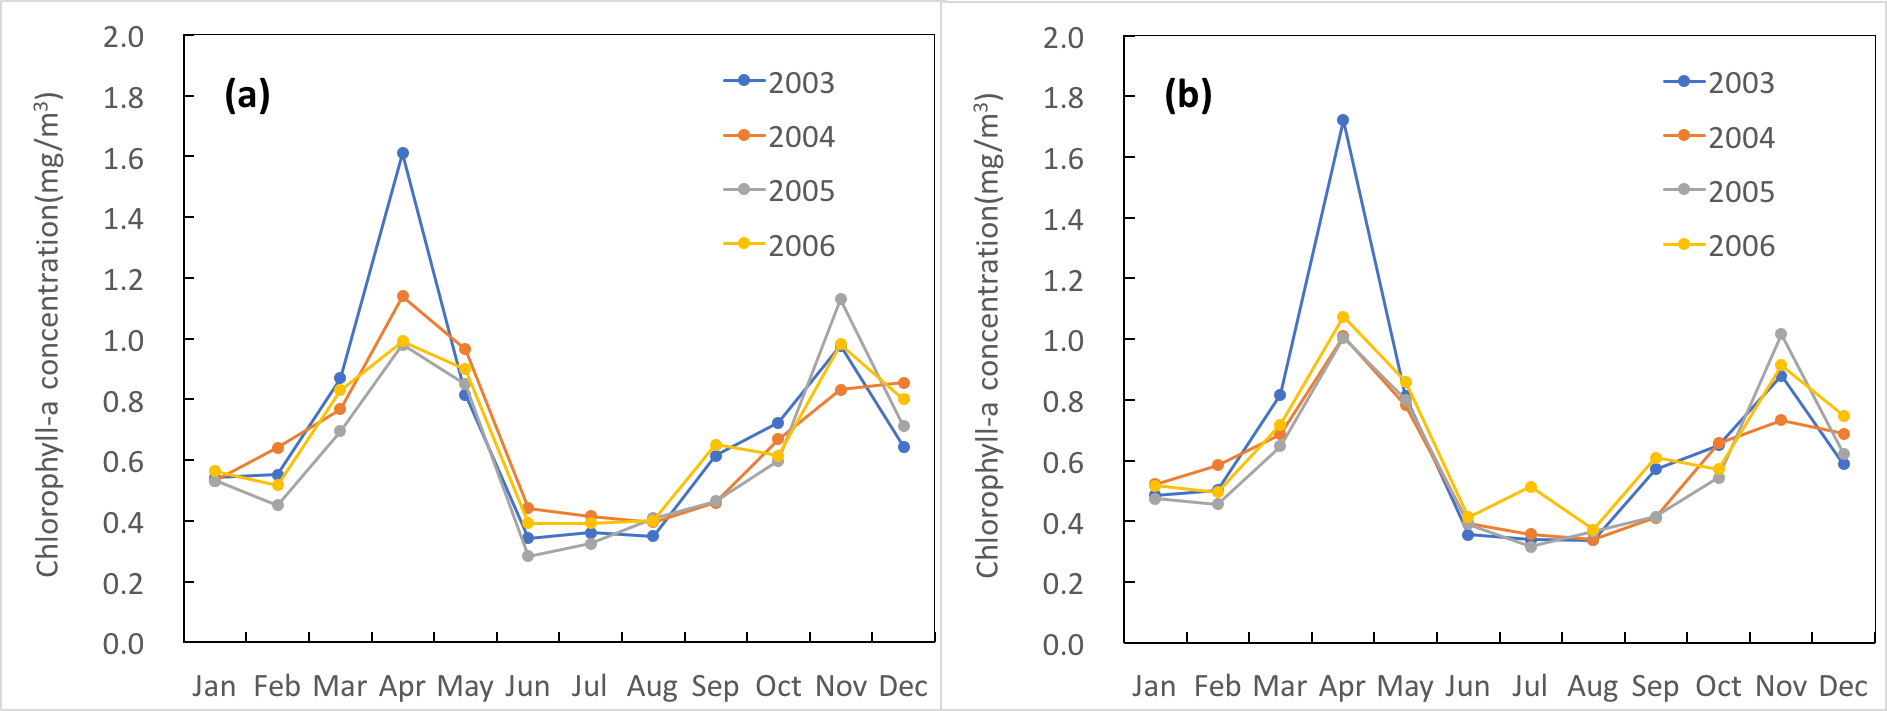
\includegraphics[width=1.0\textwidth]{../images/annualmon}\\
% 	\caption{The annual variability of monthly-mean chlorophyll-a concentration in the East Sea (Sea of Japan) from 2003 to 2006, (a) LAC (b) GAC.}
% 	\label{fig:annualmon}
% \end{figure}

%%%%%%%%%%%%%%%%%%%%%%%%%%%%%%%%%%%%%%%%%%%%%%%%%%%%%%%%%%%%%%%%%%%%%%%%%%   


\definecolor{bblue}{HTML}{4F81BD}
\definecolor{rred}{HTML}{C0504D}
\definecolor{ggreen}{HTML}{9BBB59}
\definecolor{ppurple}{HTML}{9F4C7C}

%%%%%%%%%%%%%%%%%%%%%%%%%%%%%%%%%%%%%%%%%%%%%%%%%%%%%%%%%%%%%%%%%%%%%%%%%%   
%7-1 37--1  7-1  7-1  7-1  

\begin{figure}[b]
	\begin{tikzpicture}
	\begin{axis} [
	width=1.0\textwidth,   height = 6cm, 
	major x tick style = transparent,
	xtick = data,
	%grid=major, 
	symbolic x coords={Jan, Feb, Mar, Apr, May, Jun, Jul, Aug, Sep, Oct, Nov, Dec},
	%	xlabel= Kraft $\lbrack{}$ \si{F} $\rbrack$, 
	%xmin=0, xstep=4, xmax=47,
	ylabel= {\sffamily\small chlorophyll-a concentration ($\rm mg/m^3$)},
	ymin=0,	ystep=0.5, 	%ymax=2.1,
	scaled y ticks = false,
	ymajorgrids = true,
	%nodes near coords, % data 값 표시
	% % % % % Ausrichten der Punktbeschriftung
	every node near coord/.append style={font=\scriptsize,/pgf/number format/precision=3}]
	\addplot table [x=Month, y=meanLAC_2003] {./data/mon_over00_year.csv}; \addlegendentry{\sffamily\scriptsize 2003 LAC}
	\addplot table [x=Month, y=meanGAC_2003] {./data/mon_over00_year.csv}; \addlegendentry{\sffamily\scriptsize 2003 GAC}
	%Month,YMonth,FileLAC_2003,sumLAC_2003,meanLAC_2003,medianLAC_2003,stdLAC_2003,varLAC_2003,maxLAC_2003,minLAC_2003,totalpixLAC_2003,nanpixLAC_2003,statipixLAC_2003,percentLAC_2003,fileGAC_2003,sumGAC_2003,meanGAC_2003,medianGAC_2003,stdGAC_2003,varGAC_2003,maxGAC_2003,minGAC_2003,totalpixGAC_2003,nanpixGAC_2003,statipixGAC_2003,percentGAC_2003,sumDIFF_2003,meanDIFF_2003,medianDIFF_2003,stdDIFF_2003,varDIFF_2003,maxDIFF_2003,minDIFF_2003,totalpixDIFF_2003,nanpixDIFF_2003,statipixDIFF_2003,percentDIFF_2003,
	
	%   \fill[gray,fill opacity=0.25] (axis cs:5,0) rectangle (axis cs:7,12); %Bereich einfügen
	\end{axis}
	\end{tikzpicture}
	
	\begin{tikzpicture}
	\begin{axis} [
	width=1.0\textwidth,   height = 5cm, 
	major x tick style = transparent,
	%xmin=0, xstep=4, xmax=47,
	xtick = data,
	%grid=major, 
	symbolic x coords={Jan, Feb, Mar, Apr, May, Jun, Jul, Aug, Sep, Oct, Nov, Dec},
	%	xlabel= Kraft $\lbrack{}$ \si{F} $\rbrack$, 
	%	xmin=0,
	%	xmax=15,
	ylabel= {\sffamily\small difference ($\rm mg/m^3$)},
	%ymin=-0.2,	
	ystep=0.1, 	%ymax=0.2,
	scaled y ticks = false,
	ymajorgrids = true,
	%nodes near coords, % data 값 표시
	% % % % % Ausrichten der Punktbeschriftung
	every node near coord/.append style={font=\scriptsize,/pgf/number format/precision=3},]
	[legend pos=north east]
	\addplot table [x=Month, y=meanDIFF_2003] {./data/mon_over00_year.csv}; %\addlegendentry{\sffamily\scriptsize 2003 LAC}
	
	%Month,YMonth,FileLAC_2003,sumLAC_2003,meanLAC_2003,medianLAC_2003,stdLAC_2003,varLAC_2003,maxLAC_2003,minLAC_2003,totalpixLAC_2003,nanpixLAC_2003,statipixLAC_2003,percentLAC_2003,fileGAC_2003,sumGAC_2003,meanGAC_2003,medianGAC_2003,stdGAC_2003,varGAC_2003,maxGAC_2003,minGAC_2003,totalpixGAC_2003,nanpixGAC_2003,statipixGAC_2003,percentGAC_2003,sumDIFF_2003,meanDIFF_2003,medianDIFF_2003,stdDIFF_2003,varDIFF_2003,maxDIFF_2003,minDIFF_2003,totalpixDIFF_2003,nanpixDIFF_2003,statipixDIFF_2003,percentDIFF_2003,
	
	%   \fill[gray,fill opacity=0.25] (axis cs:5,0) rectangle (axis cs:7,12); %Bereich einfügen
	\end{axis}
	\end{tikzpicture}
	
	\begin{tikzpicture}	
	\begin{axis} [
	width=1.0\textwidth,   height = 6cm, 
	major x tick style = transparent,
	xtick = data,
	symbolic x coords={Jan, Feb, Mar, Apr, May, Jun, Jul, Aug, Sep, Oct, Nov, Dec},
	ybar=4*\pgflinewidth,
	bar width=8pt,
	ymajorgrids = true,
	ylabel= {\sffamily\scriptsize Number (\%)},
	scaled y ticks = false,
	%enlarge x limits=0.25,
	ymin=0, ystep=10, %ymax=100,
	%legend cell align=left,
	%legend style={	%at={(1,1.05)},		anchor=south east, 		%column sep=1ex, 	}]
	legend pos=north east
	]
	\addplot[style={blue,fill=bblue,mark=none}] table [x=Month, y=percentLAC_2003] {./data/mon_over03_year.csv}; \addlegendentry{\sffamily\scriptsize 2003 LAC}
	\addplot[style={red,fill=rred,mark=none}] table [x=Month, y=percentGAC_2003] {./data/mon_over03_year.csv}; \addlegendentry{\sffamily\scriptsize 2003 GAC}
	
	%Month,YMonth,FileLAC_2003,sumLAC_2003,meanLAC_2003,medianLAC_2003,stdLAC_2003,varLAC_2003,maxLAC_2003,minLAC_2003,totalpixLAC_2003,nanpixLAC_2003,statipixLAC_2003,percentLAC_2003,fileGAC_2003,sumGAC_2003,meanGAC_2003,medianGAC_2003,stdGAC_2003,varGAC_2003,maxGAC_2003,minGAC_2003,totalpixGAC_2003,nanpixGAC_2003,statipixGAC_2003,percentGAC_2003,sumDIFF_2003,meanDIFF_2003,medianDIFF_2003,stdDIFF_2003,varDIFF_2003,maxDIFF_2003,minDIFF_2003,totalpixDIFF_2003,nanpixDIFF_2003,statipixDIFF_2003,percentDIFF_2003,
	\end{axis}
	\end{tikzpicture}
	
	\caption{(a) monthly mean values of chlorophyll-a concentration in 2003 using LAC (blue line) and GAC (red line) and (b) its differences between the LAC and GAC data and (c) is shown the percent of pixel number ( > 3 ) (7-1  7-1  7-1  7-1  7-1  )}
	\label{fig:diff_2003}
\end{figure}


%%%%%%%%%%%%%%%%%%%%%%%%%%%%%%%%%%%%%%%%%%%%%%%%%%%%%%%%%%%%%%%%%%%%%%%%%%   
%7-2  7-2  7-2  7-2  7-2  

\begin{figure}[h]
	\begin{tikzpicture}
	\begin{axis} [
	width=1.0\textwidth,   height = 6cm, 
	major x tick style = transparent,
	xtick = data,
	%grid=major, 
	symbolic x coords={Jan, Feb, Mar, Apr, May, Jun, Jul, Aug, Sep, Oct, Nov, Dec},
	%	xlabel= Kraft $\lbrack{}$ \si{F} $\rbrack$, 
	%xmin=0, xstep=4, xmax=47,
	ylabel= {\sffamily\small chlorophyll-a concentration ($\rm mg/m^3$)},
	ymin=0,	ystep=0.5, 	%ymax=2.1,
	scaled y ticks = false,
	ymajorgrids = true,
	%nodes near coords, % data 값 표시
	% % % % % Ausrichten der Punktbeschriftung
	every node near coord/.append style={font=\scriptsize,/pgf/number format/precision=3}]
	\addplot table [x=Month, y=meanLAC_2004] {./data/mon_over00_year.csv}; \addlegendentry{\sffamily\scriptsize 2004 LAC}
	\addplot table [x=Month, y=meanGAC_2004] {./data/mon_over00_year.csv}; \addlegendentry{\sffamily\scriptsize 2004 GAC}
	%Month,YMonth,FileLAC_2003,sumLAC_2003,meanLAC_2003,medianLAC_2003,stdLAC_2003,varLAC_2003,maxLAC_2003,minLAC_2003,totalpixLAC_2003,nanpixLAC_2003,statipixLAC_2003,percentLAC_2003,fileGAC_2003,sumGAC_2003,meanGAC_2003,medianGAC_2003,stdGAC_2003,varGAC_2003,maxGAC_2003,minGAC_2003,totalpixGAC_2003,nanpixGAC_2003,statipixGAC_2003,percentGAC_2003,sumDIFF_2003,meanDIFF_2003,medianDIFF_2003,stdDIFF_2003,varDIFF_2003,maxDIFF_2003,minDIFF_2003,totalpixDIFF_2003,nanpixDIFF_2003,statipixDIFF_2003,percentDIFF_2003,
	
	%   \fill[gray,fill opacity=0.25] (axis cs:5,0) rectangle (axis cs:7,12); %Bereich einfügen
	\end{axis}
	\end{tikzpicture}
	
	\begin{tikzpicture}
	\begin{axis} [
	width=1.0\textwidth,   height = 4cm, 
	major x tick style = transparent,
	%xmin=0, xstep=4, xmax=47,
	xtick = data,
	%grid=major, 
	symbolic x coords={Jan, Feb, Mar, Apr, May, Jun, Jul, Aug, Sep, Oct, Nov, Dec},
	%	xlabel= Kraft $\lbrack{}$ \si{F} $\rbrack$, 
	%	xmin=0,
	%	xmax=15,
	ylabel= {\sffamily\small difference ($\rm mg/m^3$)},
	%ymin=-0.2,	
	ystep=0.1, 		%ymax=0.2,
	scaled y ticks = false,
	ymajorgrids = true,
	%nodes near coords, % data 값 표시
	% % % % % Ausrichten der Punktbeschriftung
	every node near coord/.append style={font=\scriptsize,/pgf/number format/precision=3},]
	[legend pos=north east]
	\addplot table [x=Month, y=meanDIFF_2004] {./data/mon_over00_year.csv}; %\addlegendentry{\sffamily\scriptsize 2004 LAC}
	
	%Month,YMonth,FileLAC_2003,sumLAC_2003,meanLAC_2003,medianLAC_2003,stdLAC_2003,varLAC_2003,maxLAC_2003,minLAC_2003,totalpixLAC_2003,nanpixLAC_2003,statipixLAC_2003,percentLAC_2003,fileGAC_2003,sumGAC_2003,meanGAC_2003,medianGAC_2003,stdGAC_2003,varGAC_2003,maxGAC_2003,minGAC_2003,totalpixGAC_2003,nanpixGAC_2003,statipixGAC_2003,percentGAC_2003,sumDIFF_2003,meanDIFF_2003,medianDIFF_2003,stdDIFF_2003,varDIFF_2003,maxDIFF_2003,minDIFF_2003,totalpixDIFF_2003,nanpixDIFF_2003,statipixDIFF_2003,percentDIFF_2003,
	
	%   \fill[gray,fill opacity=0.25] (axis cs:5,0) rectangle (axis cs:7,12); %Bereich einfügen
	\end{axis}
	\end{tikzpicture}
	
	\begin{tikzpicture}	
	\begin{axis} [
	width=1.0\textwidth,   height = 6cm, 
	major x tick style = transparent,
	xtick = data,
	symbolic x coords={Jan, Feb, Mar, Apr, May, Jun, Jul, Aug, Sep, Oct, Nov, Dec},
	ybar=4*\pgflinewidth,
	bar width=8pt,
	ymajorgrids = true,
	ylabel= {\sffamily\small Number (\%)},
	scaled y ticks = false,
	%enlarge x limits=0.25,
	ymin=0, ystep=10, %ymax=100,
	%legend cell align=left,
	%legend style={	%at={(1,1.05)},		anchor=south east, 		%column sep=1ex, 	}]
	legend pos=north east
	]
	\addplot[style={blue,fill=bblue,mark=none}] table [x=Month, y=percentLAC_2004] {./data/mon_over03_year.csv}; \addlegendentry{\sffamily\scriptsize 2004 LAC}
	\addplot[style={red,fill=rred,mark=none}] table [x=Month, y=percentGAC_2004] {./data/mon_over03_year.csv}; \addlegendentry{\sffamily\scriptsize 2004 GAC}
	
	%Month,YMonth,FileLAC_2003,sumLAC_2003,meanLAC_2003,medianLAC_2003,stdLAC_2003,varLAC_2003,maxLAC_2003,minLAC_2003,totalpixLAC_2003,nanpixLAC_2003,statipixLAC_2003,percentLAC_2003,fileGAC_2003,sumGAC_2003,meanGAC_2003,medianGAC_2003,stdGAC_2003,varGAC_2003,maxGAC_2003,minGAC_2003,totalpixGAC_2003,nanpixGAC_2003,statipixGAC_2003,percentGAC_2003,sumDIFF_2003,meanDIFF_2003,medianDIFF_2003,stdDIFF_2003,varDIFF_2003,maxDIFF_2003,minDIFF_2003,totalpixDIFF_2003,nanpixDIFF_2003,statipixDIFF_2003,percentDIFF_2003,
	\end{axis}
	\end{tikzpicture}
	
	\caption{(a) monthly mean values of chlorophyll-a concentration in 2004 using LAC (blue line) and GAC (red line) and (b) its differences between the LAC and GAC data and (c) is shown the percent of pixel number ( > 3 ) (7-2  7-2  7-2  7-2  7-2  )}
	\label{fig:diff_2004}
\end{figure}


%%%%%%%%%%%%%%%%%%%%%%%%%%%%%%%%%%%%%%%%%%%%%%%%%%%%%%%%%%%%%%%%%%%%%%%%%%   
%7-3  7-3  7-3  7-3  7-3  

\begin{figure}[h]
	\begin{tikzpicture}
	\begin{axis} [
	width=1.0\textwidth,   height = 6cm, 
	major x tick style = transparent,
	xtick = data,
	%grid=major, 
	symbolic x coords={Jan, Feb, Mar, Apr, May, Jun, Jul, Aug, Sep, Oct, Nov, Dec},
	%	xlabel= Kraft $\lbrack{}$ \si{F} $\rbrack$, 
	%xmin=0, xstep=4, xmax=47,
	ylabel= {\sffamily\small chlorophyll-a concentration ($\rm mg/m^3$)},
	ymin=0,	ystep=0.5, 	%ymax=2.1,
	scaled y ticks = false,
	ymajorgrids = true,
	%nodes near coords, % data 값 표시
	% % % % % Ausrichten der Punktbeschriftung
	every node near coord/.append style={font=\scriptsize,/pgf/number format/precision=3}]
	\addplot table [x=Month, y=meanLAC_2005] {./data/mon_over00_year.csv}; \addlegendentry{\sffamily\scriptsize 2005 LAC}
	\addplot table [x=Month, y=meanGAC_2005] {./data/mon_over00_year.csv}; \addlegendentry{\sffamily\scriptsize 2005 GAC}
	%Month,YMonth,FileLAC_2003,sumLAC_2003,meanLAC_2003,medianLAC_2003,stdLAC_2003,varLAC_2003,maxLAC_2003,minLAC_2003,totalpixLAC_2003,nanpixLAC_2003,statipixLAC_2003,percentLAC_2003,fileGAC_2003,sumGAC_2003,meanGAC_2003,medianGAC_2003,stdGAC_2003,varGAC_2003,maxGAC_2003,minGAC_2003,totalpixGAC_2003,nanpixGAC_2003,statipixGAC_2003,percentGAC_2003,sumDIFF_2003,meanDIFF_2003,medianDIFF_2003,stdDIFF_2003,varDIFF_2003,maxDIFF_2003,minDIFF_2003,totalpixDIFF_2003,nanpixDIFF_2003,statipixDIFF_2003,percentDIFF_2003,
	
	%   \fill[gray,fill opacity=0.25] (axis cs:5,0) rectangle (axis cs:7,12); %Bereich einfügen
	\end{axis}
	\end{tikzpicture}
	
	\begin{tikzpicture}
	\begin{axis} [
	width=1.0\textwidth,   height = 5cm, 
	major x tick style = transparent,
	%xmin=0, xstep=4, xmax=47,
	xtick = data,
	%grid=major, 
	symbolic x coords={Jan, Feb, Mar, Apr, May, Jun, Jul, Aug, Sep, Oct, Nov, Dec},
	%	xlabel= Kraft $\lbrack{}$ \si{F} $\rbrack$, 
	%	xmin=0,
	%	xmax=15,
	ylabel= {\sffamily\small difference ($\rm mg/m^3$)},
	%ymin=-0.2,	
	ystep=0.1, 	%ymax=0.2,
	scaled y ticks = false,
	ymajorgrids = true,
	%nodes near coords, % data 값 표시
	% % % % % Ausrichten der Punktbeschriftung
	every node near coord/.append style={font=\scriptsize,/pgf/number format/precision=3},]
	[legend pos=north east]
	\addplot table [x=Month, y=meanDIFF_2005] {./data/mon_over00_year.csv}; %\addlegendentry{\sffamily\scriptsize 2005 LAC}
	
	%Month,YMonth,FileLAC_2003,sumLAC_2003,meanLAC_2003,medianLAC_2003,stdLAC_2003,varLAC_2003,maxLAC_2003,minLAC_2003,totalpixLAC_2003,nanpixLAC_2003,statipixLAC_2003,percentLAC_2003,fileGAC_2003,sumGAC_2003,meanGAC_2003,medianGAC_2003,stdGAC_2003,varGAC_2003,maxGAC_2003,minGAC_2003,totalpixGAC_2003,nanpixGAC_2003,statipixGAC_2003,percentGAC_2003,sumDIFF_2003,meanDIFF_2003,medianDIFF_2003,stdDIFF_2003,varDIFF_2003,maxDIFF_2003,minDIFF_2003,totalpixDIFF_2003,nanpixDIFF_2003,statipixDIFF_2003,percentDIFF_2003,
	
	%   \fill[gray,fill opacity=0.25] (axis cs:5,0) rectangle (axis cs:7,12); %Bereich einfügen
	\end{axis}
	\end{tikzpicture}
	
	\begin{tikzpicture}	
	\begin{axis} [
	width=1.0\textwidth,   height = 6cm, 
	major x tick style = transparent,
	xtick = data,
	symbolic x coords={Jan, Feb, Mar, Apr, May, Jun, Jul, Aug, Sep, Oct, Nov, Dec},
	ybar=4*\pgflinewidth,
	bar width=8pt,
	ymajorgrids = true,
	ylabel= {\sffamily\small Number (\%)},
	scaled y ticks = false,
	%enlarge x limits=0.25,
	ymin=0, ystep=10, %ymax=100,
	%legend cell align=left,
	%legend style={	%at={(1,1.05)},		anchor=south east, 		%column sep=1ex, 	}]
	legend pos=north east
	]
	\addplot[style={blue,fill=bblue,mark=none}] table [x=Month, y=percentLAC_2005] {./data/mon_over03_year.csv}; \addlegendentry{\sffamily\scriptsize 2005 LAC}
	\addplot[style={red,fill=rred,mark=none}] table [x=Month, y=percentGAC_2005] {./data/mon_over03_year.csv}; \addlegendentry{\sffamily\scriptsize 2005 GAC}
	
	%Month,YMonth,FileLAC_2003,sumLAC_2003,meanLAC_2003,medianLAC_2003,stdLAC_2003,varLAC_2003,maxLAC_2003,minLAC_2003,totalpixLAC_2003,nanpixLAC_2003,statipixLAC_2003,percentLAC_2003,fileGAC_2003,sumGAC_2003,meanGAC_2003,medianGAC_2003,stdGAC_2003,varGAC_2003,maxGAC_2003,minGAC_2003,totalpixGAC_2003,nanpixGAC_2003,statipixGAC_2003,percentGAC_2003,sumDIFF_2003,meanDIFF_2003,medianDIFF_2003,stdDIFF_2003,varDIFF_2003,maxDIFF_2003,minDIFF_2003,totalpixDIFF_2003,nanpixDIFF_2003,statipixDIFF_2003,percentDIFF_2003,
	\end{axis}
	\end{tikzpicture}
	
	\caption{(a) monthly mean values of chlorophyll-a concentration in 2005 using LAC (blue line) and GAC (red line) and (b) its differences between the LAC and GAC data and (c) is shown the percent of pixel number ( > 3 ) (7-3  7-3  7-3  7-3  7-3  )}
	\label{fig:diff_2005}
\end{figure}

%%%%%%%%%%%%%%%%%%%%%%%%%%%%%%%%%%%%%%%%%%%%%%%%%%%%%%%%%%%%%%%%%%%%%%%%%%   
%7-4  7-4  7-4  7-4  7-4  

\begin{figure}[h]
	\begin{tikzpicture}
	\begin{axis} [
	width=1.0\textwidth,   height = 6cm, 
	major x tick style = transparent,
	xtick = data,
	%grid=major, 
	symbolic x coords={Jan, Feb, Mar, Apr, May, Jun, Jul, Aug, Sep, Oct, Nov, Dec},
	%	xlabel= Kraft $\lbrack{}$ \si{F} $\rbrack$, 
	%xmin=0, xstep=4, xmax=47,
	ylabel= {\sffamily\small chlorophyll-a concentration ($\rm mg/m^3$)},
	ymin=0,	ystep=0.5, 	%ymax=2.1,
	scaled y ticks = false,
	ymajorgrids = true,
	%nodes near coords, % data 값 표시
	% % % % % Ausrichten der Punktbeschriftung
	every node near coord/.append style={font=\scriptsize,/pgf/number format/precision=3}]
	\addplot table [x=Month, y=meanLAC_2006] {./data/mon_over00_year.csv}; \addlegendentry{\sffamily\scriptsize 2006 LAC}
	\addplot table [x=Month, y=meanGAC_2006] {./data/mon_over00_year.csv}; \addlegendentry{\sffamily\scriptsize 2006 GAC}
	%Month,YMonth,FileLAC_2003,sumLAC_2003,meanLAC_2003,medianLAC_2003,stdLAC_2003,varLAC_2003,maxLAC_2003,minLAC_2003,totalpixLAC_2003,nanpixLAC_2003,statipixLAC_2003,percentLAC_2003,fileGAC_2003,sumGAC_2003,meanGAC_2003,medianGAC_2003,stdGAC_2003,varGAC_2003,maxGAC_2003,minGAC_2003,totalpixGAC_2003,nanpixGAC_2003,statipixGAC_2003,percentGAC_2003,sumDIFF_2003,meanDIFF_2003,medianDIFF_2003,stdDIFF_2003,varDIFF_2003,maxDIFF_2003,minDIFF_2003,totalpixDIFF_2003,nanpixDIFF_2003,statipixDIFF_2003,percentDIFF_2003,
	
	%   \fill[gray,fill opacity=0.25] (axis cs:5,0) rectangle (axis cs:7,12); %Bereich einfügen
	\end{axis}
	\end{tikzpicture}
	
	\begin{tikzpicture}
	\begin{axis} [
	width=1.0\textwidth,   height = 5cm, 
	major x tick style = transparent,
	%xmin=0, xstep=4, xmax=47,
	xtick = data,
	%grid=major, 
	%\sffamily\tiny
	{symbolic x coords={Jan, Feb, Mar, Apr, May, Jun, Jul, Aug, Sep, Oct, Nov, Dec}},
	%	xlabel= Kraft $\lbrack{}$ \si{F} $\rbrack$, 
	%	xmin=0,
	%	xmax=15,
	ylabel= {\sffamily\small difference ($\rm mg/m^3$)},
	%ymin=-0.2,	
	ystep=0.1, 	%ymax=0.2,
	scaled y ticks = false,
	ymajorgrids = true,
	y tick label style={/pgf/number format/.cd,sci,precision=5}]
	%nodes near coords, % data 값 표시
	% % % % % Ausrichten der Punktbeschriftung
	every node near coord/.append style={font=\scriptsize,/pgf/number format/precision=1},]
	[legend pos=north east]
	\addplot table [x=Month, y=meanDIFF_2006] {./data/mon_over00_year.csv}; %\addlegendentry{\sffamily\scriptsize 2006 LAC}
	
	%Month,YMonth,FileLAC_2003,sumLAC_2003,meanLAC_2003,medianLAC_2003,stdLAC_2003,varLAC_2003,maxLAC_2003,minLAC_2003,totalpixLAC_2003,nanpixLAC_2003,statipixLAC_2003,percentLAC_2003,fileGAC_2003,sumGAC_2003,meanGAC_2003,medianGAC_2003,stdGAC_2003,varGAC_2003,maxGAC_2003,minGAC_2003,totalpixGAC_2003,nanpixGAC_2003,statipixGAC_2003,percentGAC_2003,sumDIFF_2003,meanDIFF_2003,medianDIFF_2003,stdDIFF_2003,varDIFF_2003,maxDIFF_2003,minDIFF_2003,totalpixDIFF_2003,nanpixDIFF_2003,statipixDIFF_2003,percentDIFF_2003,
	
	%   \fill[gray,fill opacity=0.25] (axis cs:5,0) rectangle (axis cs:7,12); %Bereich einfügen
	\end{axis}
	\end{tikzpicture}
	
	\begin{tikzpicture}	
	\begin{axis} [
	width=1.0\textwidth,   height = 6cm, 
	major x tick style = transparent,
	xtick = data,
	symbolic x coords={Jan, Feb, Mar, Apr, May, Jun, Jul, Aug, Sep, Oct, Nov, Dec},
	ybar=4*\pgflinewidth,
	bar width=8pt,
	ymajorgrids = true,
	ylabel= {\sffamily\small Number (\%)},
	scaled y ticks = false,
	%enlarge x limits=0.25,
	ymin=0, ystep=10, %ymax=100,
	%legend cell align=left,
	%legend style={	%at={(1,1.05)},		anchor=south east, 		%column sep=1ex, 	}]
	legend pos=north east
	]
	\addplot[style={blue,fill=bblue,mark=none}] table [x=Month, y=percentLAC_2006] {./data/mon_over03_year.csv}; \addlegendentry{\sffamily\scriptsize 2006 LAC}
	\addplot[style={red,fill=rred,mark=none}] table [x=Month, y=percentGAC_2006] {./data/mon_over03_year.csv}; \addlegendentry{\sffamily\scriptsize 2006 GAC}
	
	%Month,YMonth,FileLAC_2003,sumLAC_2003,meanLAC_2003,medianLAC_2003,stdLAC_2003,varLAC_2003,maxLAC_2003,minLAC_2003,totalpixLAC_2003,nanpixLAC_2003,statipixLAC_2003,percentLAC_2003,fileGAC_2003,sumGAC_2003,meanGAC_2003,medianGAC_2003,stdGAC_2003,varGAC_2003,maxGAC_2003,minGAC_2003,totalpixGAC_2003,nanpixGAC_2003,statipixGAC_2003,percentGAC_2003,sumDIFF_2003,meanDIFF_2003,medianDIFF_2003,stdDIFF_2003,varDIFF_2003,maxDIFF_2003,minDIFF_2003,totalpixDIFF_2003,nanpixDIFF_2003,statipixDIFF_2003,percentDIFF_2003,
	\end{axis}
	\end{tikzpicture}
	
	\caption{(a) monthly mean values of chlorophyll-a concentration in 2006 using LAC (blue line) and GAC (red line) and (b) its differences between the LAC and GAC data and (c) is shown the percent of pixel number ( > 3 ) (7-4  7-4  7-4  7-4  7-4  )}
	\label{fig:diff_2006}
\end{figure}



The annual variability of chlorophyll-a concentration in the East Sea (Sea of Japan) from 2003 - 2006 is shown in Figure 1 and Figure 2. Both the LAC data and the GAC data have similar tendency, showing peaks on spring (April) and fall (November). The maximum/minimum value of LAC and GAC data was each 1.61 $\rm mg/m^3$ / 0.28 $\rm mg/m^3$, and 1.72 $\rm mg/m^3$ / 0.32 $\rm mg/m^3$. The difference between the two data was not ignorable. This infers that the effect of spatial resolution on the data has to be considered.
It is shown in Figure \ref{fig:annualmon} that the annual variability of monthly-mean chlorophyll-a concentration in the East Sea (Sea of Japan) from 2003 to 2006, (a) LAC (b) GAC.

 
 
%%%%%%%%%%%%%%%%%%%%%%%%%%%%%%%%%%%%%%%%%%%%%%%%%%%%%%%%%%%%%%%%%%%%%%%% 
% \begin{figure}[b]
%	\centering
%	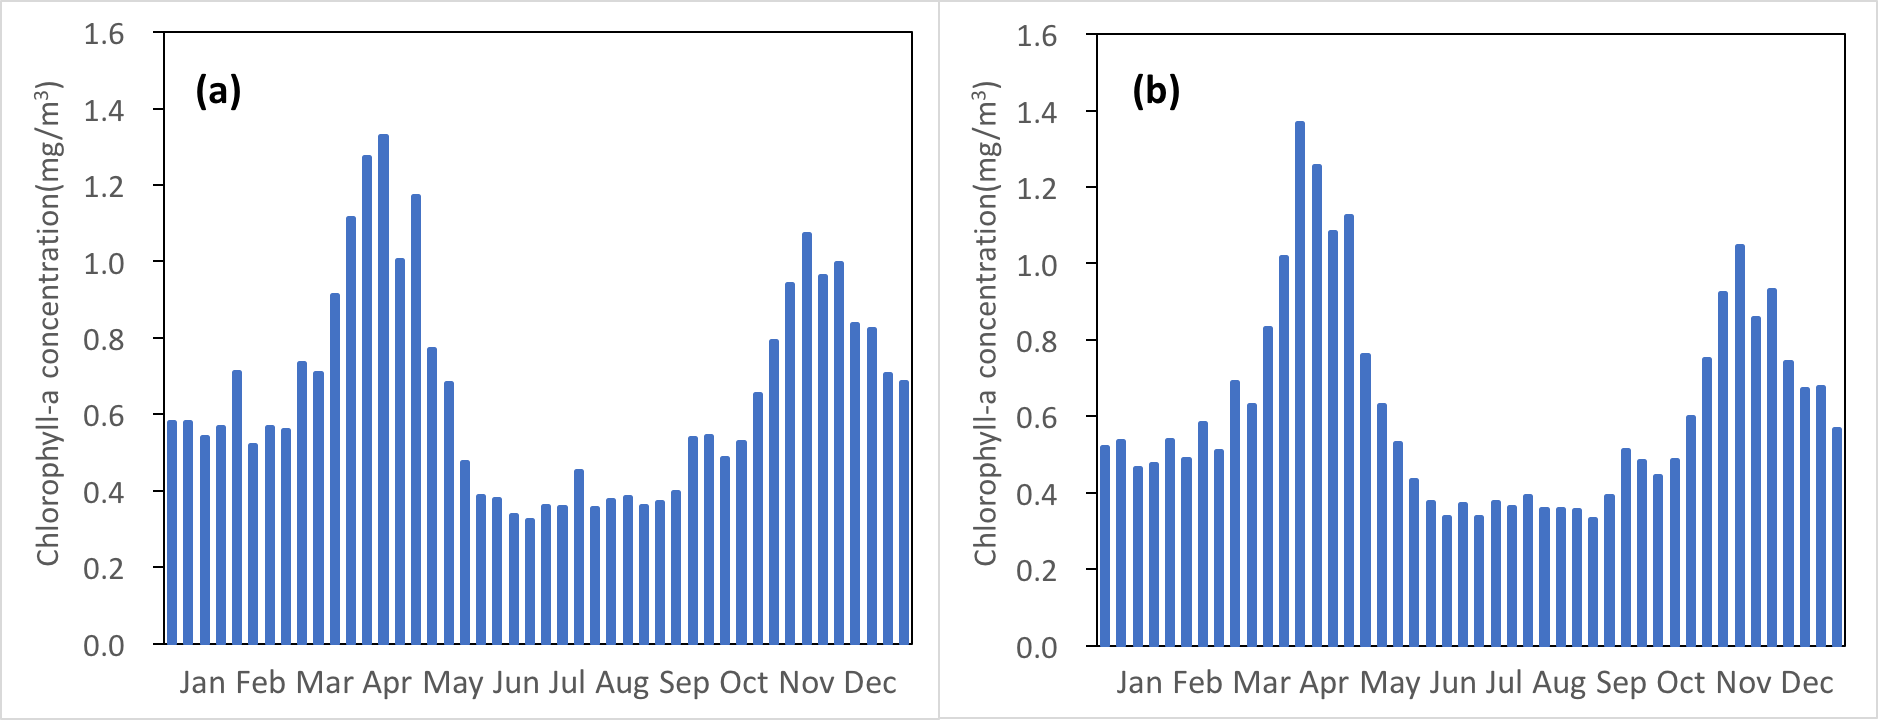
\includegraphics[width=1.0\textwidth]{../images/annualwky}\\
%	\caption{The annual variability of 8-day-mean chlorophyll-a concentration in the East Sea (Sea of Japan), (a) LAC (b) GAC. Each 8-day-mean data is average of data from 2003 to 2006.}
%	\label{fig:annuawkly}
%\end{figure}


  
  The annual variability of 8-day-mean chlorophyll-a concentration in the East Sea (Sea of Japan) from 2003 to 2006 is shown in Figure 3 and Figure 4. This result allowed more concrete analysis of the data. The spring peak had 1.2 - 1.3 $\rm mg/m^3$ of chlorophyll-a concentration and was higher than the fall peak which had 0.9 - 1.0 $\rm mg/m^3$. Winter had a higher concentration (0.6 $\rm mg/m^3$) compared to summer (0.4 $\rm mg/m^3$). The chlorophyll-a concentration in the East Sea (Sea of Japan) had clear seasonal differences. Both the LAC data and the GAC data were sufficient to show the seasonal differences. However, even though the 8-day-mean data was created using average of 4 years chlorophyll-a concentration data, the time of maximum concentration was different. 
  
  Part of the LAC data (2004 46th 8-day-mean, 2005 11th 8-day-mean, 2005 31th 8-day-mean) had been lost due to satellite failures. The data for these periods were substituted with the average of the adjacent data, which did not have a significant effect on the tendency. Consequently, the error was ignorable.
 
\begin{figure}[h]
	\begin{tikzpicture}
	\begin{axis} 
	[ width=0.98\textwidth,   height = 7cm, 
	major x tick style = transparent,
	xtick = data,
	%grid=major, 
	%zeichnet Koordinatengitter
	xmin=0, xstep=4, xmax=47,
	%symbolic x coords={5, 10, 15, 20, 25,30, 35, 40, 45, 50},
	%xlabel= Kraft $\lbrack{}$ \si{F} $\rbrack$, 
	ylabel= {\sffamily\small chlorophyll-a concentration ($\rm mg/m^3$)},
ymin=0,	ystep=0.5, 	ymax=3.1,
scaled y ticks = false,
%nodes near coords, % data 값 표시
% % % % % Ausrichten der Punktbeschriftung
every node near coord/.append style={font=\scriptsize,/pgf/number format/precision=3}]
[legend pos=north east]
\addplot table [x=Week, y=2003] {./data/wkyLAC.csv}; \addlegendentry{\sffamily\scriptsize 2003}
\addplot table [x=Week, y=2004] {./data/wkyLAC.csv}; \addlegendentry{\sffamily\scriptsize 2004}
\addplot table [x=Week, y=2005] {./data/wkyLAC.csv}; \addlegendentry{\sffamily\scriptsize 2005}
\addplot table [x=Week, y=2006] {./data/wkyLAC.csv}; \addlegendentry{\sffamily\scriptsize 2006}
%   \fill[gray,fill opacity=0.25] (axis cs:5,0) rectangle (axis cs:7,12); %Bereich einfügen
\end{axis}
\end{tikzpicture}

\begin{tikzpicture}
\begin{axis} 
[ width=0.98\textwidth,   height = 7cm, 
major x tick style = transparent,
xtick = data,
%grid=major, 
%zeichnet Koordinatengitter
xmin=0, xstep=4, xmax=47,
%symbolic x coords={Jan, Feb, Mar, Apr, May, Jun, Jul, Aug, Sep, Oct, Nov, Dec},
%xlabel= Kraft $\lbrack{}$ \si{F} $\rbrack$, 
ylabel= {\sffamily\small chlorophyll-a concentration ($\rm mg/m^3$)},
ymin=0,	ystep=0.5, 	ymax=3.1,
scaled y ticks = false,
%nodes near coords, % data 값 표시
% % % % % Ausrichten der Punktbeschriftung
every node near coord/.append style={font=\scriptsize,/pgf/number format/precision=3}]
[legend pos=north east]
\addplot table [x=Week, y=2003] {./data/wkyGAC.csv}; \addlegendentry{\sffamily\scriptsize 2003}
\addplot table [x=Week, y=2004] {./data/wkyGAC.csv}; \addlegendentry{\sffamily\scriptsize 2004}
\addplot table [x=Week, y=2005] {./data/wkyGAC.csv}; \addlegendentry{\sffamily\scriptsize 2005}
\addplot table [x=Week, y=2006] {./data/wkyGAC.csv}; \addlegendentry{\sffamily\scriptsize 2006}
%   \fill[gray,fill opacity=0.25] (axis cs:5,0) rectangle (axis cs:7,12); %Bereich einfügen

\end{axis}
\end{tikzpicture}
\caption{The annual variability of 8-day-mean chlorophyll-a concentration in the East Sea (Sea of Japan), (a) LAC (b) GAC. Each 8-day-mean data is average of data from 2003 to 2006.}
\label{fig:annuawkly}
\end{figure}


\newpage
\newpage

\subsection{The Effect of Spatial Resolution on the Data}
 
To find the effect of spatial resolution on the data, the histograms of LAC data and the GAC data of April, 2003 are compared. The histogram of GAC data showed more discontinuous shape compared to the LAC data in Figure \ref{fig:monHIS}. From the fact that a histogram of real data has continuous shape, it can be inferred that using LAC data is more accurate than using GAC data. The histogram of GAC data also shows more pixels with over $\rm mg/m^3$ of chlorophyll-a concentration with sporadic distribution. These pixels are the speckles from previous researches (Chae, H. J., and Park, K., 2009; Hu, C., Carder, K. L., and Muller-Karger, F. E., 2001). The number of speckles also show that LAC data is more appropriate for studying chlorophyll-a concentration \cite{chae2009characteristics,hu2001precise}.
  
\begin{figure}[h]
	\centering
	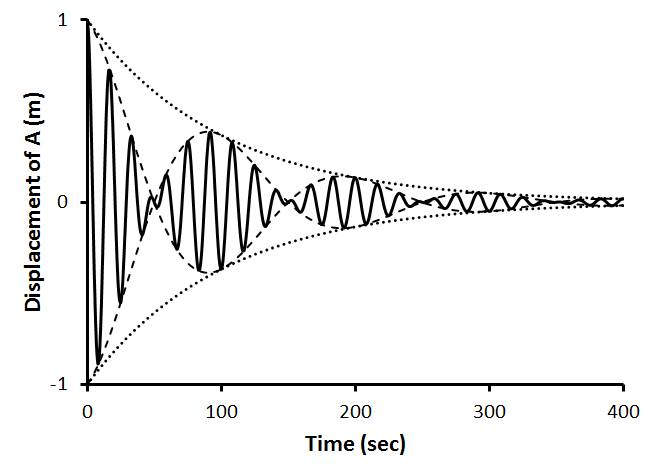
\includegraphics[width=0.8\textwidth]{../images/monHIS}\\
	\caption{The monthly chlorophyll-a mean histogram in the East Sea (Sea of Japan) on April, 2003, (a) LAC (b) GAC.}
	\label{fig:monHIS}
\end{figure}
 
In Figure\ref{fig:monHISHI}, part of the data with high chlorophyll-a concentration is enlarged to compare LAC data and GAC data. LAC data has 6 pixels over $\rm mg/m^3$, while GAC data has more than 100 pixels over 10 $\rm mg/m^3$. Such result is shown since one high-concentration value in GAC data affects a larger area compared to LAC because of its low resolution.
In Figure\ref{fig:monHISSPEC}, a part of the data with speckles is enlarged to compare LAC data and GAC data. GAC data has a larger size of speckle due to its low resolution, which causes more errors. Even if the speckles of the GAC data is corrected, it will correct a larger area compared to LAC causing a more gap between the real value. In addition, even with the speckle correction applied using corrected LAC data will be more accurate.
    
  \begin{figure}[h]
  	\centering
  	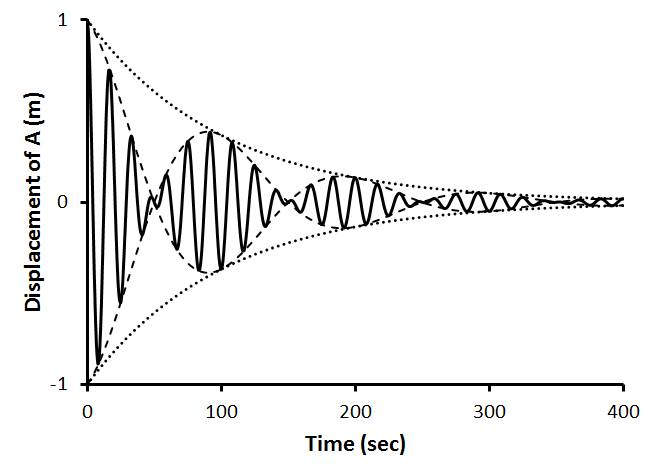
\includegraphics[width=0.8\textwidth]{../images/monHISHI}\\
  	\caption{The monthly chlorophyll-a mean distribution in the East Sea (Sea of Japan) on April, 2003, (a) LAC (b) GAC. Enlarged an area with high concentrations of chlorophyll-a.}
  	\label{fig:monHISHI}x
  \end{figure}
  
    \begin{figure}[h]
  	\centering
  	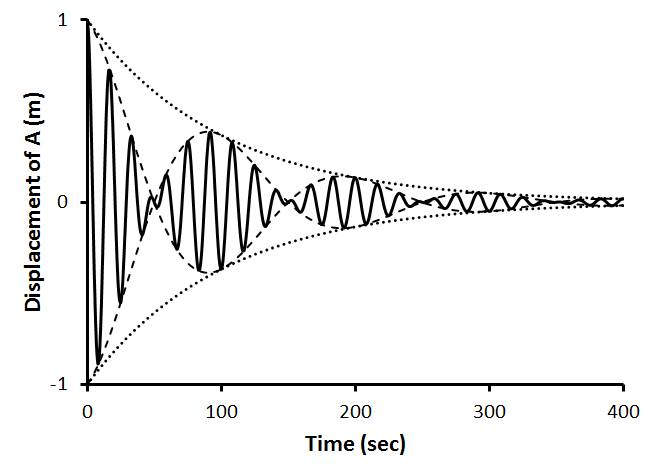
\includegraphics[width=0.8\textwidth]{../images/monHISSPEC}\\
  	\caption{The monthly chlorophyll-a mean distribution in the East Sea (Sea of Japan) on April, 2003, (a) LAC (b) GAC. Enlarged an area with speckles.}
  	\label{fig:monHISSPEC}
  \end{figure}
  